% =====================================================================
% habitID-Net -- IEEE conference format (IEEEtran)
% Compile: pdflatex habitID_Net_paper.tex  (run twice)   [Overleaf works as-is]
% All results are placeholders: replace every \TBD{...} with real numbers
% from your own runs. Verify every reference before submission.
% =====================================================================
\documentclass[conference]{IEEEtran}

\usepackage{cite}
\usepackage{amsmath,amssymb,amsfonts}
\usepackage{algorithm}
\usepackage{algpseudocode}
\usepackage{graphicx}
\usepackage{booktabs}
\usepackage{textcomp}
\usepackage{xcolor}
\usepackage{url}

% Placeholder macro: renders in red so unfilled results are impossible to miss
\newcommand{\TBD}[1]{\textcolor{red}{[#1]}}
\newcommand{\hid}{habitID}
% generated by scripts/10_make_paper_assets.py from results/ only
\newcommand{\Auchabitidv}{0.756}
\newcommand{\AucSdhabitidv}{0.009}
\newcommand{\Tprhabitidv}{0.185}
\newcommand{\PrAuchabitidv}{0.122}
\newcommand{\Aucgateonly}{0.500}
\newcommand{\AucSdgateonly}{0.000}
\newcommand{\Tprgateonly}{0.000}
\newcommand{\PrAucgateonly}{0.010}
\newcommand{\Auclrhandcrafted}{0.786}
\newcommand{\AucSdlrhandcrafted}{0.014}
\newcommand{\Tprlrhandcrafted}{0.450}
\newcommand{\PrAuclrhandcrafted}{0.226}
\newcommand{\Aucgbthandcrafted}{0.891}
\newcommand{\AucSdgbthandcrafted}{0.007}
\newcommand{\Tprgbthandcrafted}{0.724}
\newcommand{\PrAucgbthandcrafted}{0.725}
\newcommand{\Aucisolationforest}{0.477}
\newcommand{\AucSdisolationforest}{0.027}
\newcommand{\Tprisolationforest}{0.007}
\newcommand{\PrAucisolationforest}{0.010}
\newcommand{\Auconeclasssvm}{0.472}
\newcommand{\AucSdoneclasssvm}{0.023}
\newcommand{\Tproneclasssvm}{0.009}
\newcommand{\PrAuconeclasssvm}{0.010}
\newcommand{\Aucscaledmanhattan}{0.478}
\newcommand{\AucSdscaledmanhattan}{0.034}
\newcommand{\Tprscaledmanhattan}{0.007}
\newcommand{\PrAucscaledmanhattan}{0.010}
\newcommand{\Aucnoprior}{0.836}
\newcommand{\AucSdnoprior}{0.035}
\newcommand{\Tprnoprior}{0.635}
\newcommand{\PrAucnoprior}{0.634}
\newcommand{\Aucnoadv}{0.872}
\newcommand{\AucSdnoadv}{0.015}
\newcommand{\Tprnoadv}{0.667}
\newcommand{\PrAucnoadv}{0.670}
\newcommand{\Auctypingonly}{0.532}
\newcommand{\AucSdtypingonly}{0.043}
\newcommand{\Tprtypingonly}{0.013}
\newcommand{\PrAuctypingonly}{0.012}
\newcommand{\Aucmotiononly}{0.717}
\newcommand{\AucSdmotiononly}{0.009}
\newcommand{\Tprmotiononly}{0.362}
\newcommand{\PrAucmotiononly}{0.351}
\newcommand{\Aucotponly}{0.751}
\newcommand{\AucSdotponly}{0.005}
\newcommand{\Tprotponly}{0.476}
\newcommand{\PrAucotponly}{0.484}
\newcommand{\Auchabitidnet}{0.833}
\newcommand{\AucSdhabitidnet}{0.035}
\newcommand{\Tprhabitidnet}{0.631}
\newcommand{\PrAuchabitidnet}{0.632}
\newcommand{\dAucHabitidv}{+0.091}
\newcommand{\dAucNoprior}{-0.001}
\newcommand{\dAucNoadv}{-0.019}
\newcommand{\dAucGbthandcrafted}{-0.044}
\newcommand{\dAucLrhandcrafted}{+0.061}
\newcommand{\LofofullWorst}{0.647}
\newcommand{\LofofullWorstFam}{A}
\newcommand{\LofonoadvWorst}{0.614}
\newcommand{\LofonoadvWorstFam}{A}
\newcommand{\ConfLofoACov}{0.764}
\newcommand{\ConfLofoBCov}{0.838}
\newcommand{\ConfLofoCCov}{0.710}
\newcommand{\ConfLofoDCov}{0.742}
\newcommand{\AlphaTyping}{0.343}
\newcommand{\AlphaMotion}{0.310}
\newcommand{\AlphaOtp}{0.395}
\newcommand{\PriorDist}{0.165}
\newcommand{\AlphaZeroTyping}{0.417}
\newcommand{\AlphaZeroMotion}{0.333}
\newcommand{\AlphaZeroOtp}{0.250}
\newcommand{\DstarAuc}{0.982}
\newcommand{\DstarFlag}{0.947}
\newcommand{\AlphaTypingFull}{0.329}
\newcommand{\PerTypeFullAll}{0.969}
\newcommand{\PerTypeFullTyping}{0.502}
\newcommand{\PerTypeFullMotion}{0.834}
\newcommand{\PerTypeFullOtp}{0.904}
\newcommand{\ShareSingleSignal}{60}
\newcommand{\TsFamA}{0.998}
\newcommand{\OrigFamA}{0.557}
\newcommand{\TsFamB}{0.781}
\newcommand{\OrigFamB}{0.542}
\newcommand{\TsFamC}{0.508}
\newcommand{\OrigFamC}{0.484}
\newcommand{\TsFamD}{0.517}
\newcommand{\OrigFamD}{0.487}
\newcommand{\TsPooled}{0.884}
\newcommand{\TsEce}{0.028}
\newcommand{\OrigPooledEce}{0.034}
\newcommand{\GbtPooledEce}{0.022}
\newcommand{\GbtPooledAucP}{0.890}
\newcommand{\OrigPooledAucP}{0.847}
\newcommand{\PoolHabAuc}{0.847}
\newcommand{\PoolHabLo}{0.836}
\newcommand{\PoolHabHi}{0.858}
\newcommand{\PoolGbtAuc}{0.891}
\newcommand{\PoolGbtLo}{0.884}
\newcommand{\PoolGbtHi}{0.897}
\newcommand{\PoolNoAdvAuc}{0.866}
\newcommand{\PoolNoAdvLo}{0.856}
\newcommand{\PoolNoAdvHi}{0.876}
\newcommand{\PoolVAuc}{0.756}
\newcommand{\PoolVLo}{0.740}
\newcommand{\PoolVHi}{0.771}
\newcommand{\LofoHabFamA}{0.647}
\newcommand{\LofoGbtFamA}{0.490}
\newcommand{\LofoGbtFamB}{0.900}
\newcommand{\LofoHabFamB}{0.710}
\newcommand{\AbstainLo}{53}
\newcommand{\AbstainHi}{65}
\newcommand{\CovHumanFive}{0.932}
\newcommand{\CovBotFive}{0.954}
\newcommand{\LofoCovTen}{0.764}
\newcommand{\LofoCovFive}{0.884}
\newcommand{\EceRawFull}{0.041}
\newcommand{\EceTsFull}{0.037}
\newcommand{\EceGbt}{0.023}
\newcommand{\XferCmuToKrOn}{0.252}
\newcommand{\XferCmuToKrOff}{0.257}
\newcommand{\XferCmuToKrPds}{0.289}
\newcommand{\XferInCmuToKr}{0.775}
\newcommand{\XferKrToCmuOn}{0.456}
\newcommand{\XferKrToCmuOff}{0.441}
\newcommand{\XferKrToCmuPds}{0.642}
\newcommand{\XferInKrToCmu}{0.807}
\newcommand{\NoOtpAuc}{0.715}
\newcommand{\NoOtpAucSd}{0.021}
\newcommand{\LrNoOtpAuc}{0.685}
\newcommand{\GbtNoOtpAuc}{0.783}
\newcommand{\GbtNoOtpAucSd}{0.008}
\newcommand{\XferCMUKeyRecsonCross}{0.252}
\newcommand{\XferCMUKeyRecsonIn}{0.775}
\newcommand{\XferKeyRecsCMUonCross}{0.456}
\newcommand{\XferKeyRecsCMUonIn}{0.807}
\newcommand{\XferCMUKeyRecsoffCross}{0.257}
\newcommand{\XferCMUKeyRecsoffIn}{0.759}
\newcommand{\XferCMUKeyRecspdsCross}{0.289}
\newcommand{\XferCMUKeyRecspdsIn}{0.775}
\newcommand{\XferKeyRecsCMUoffCross}{0.441}
\newcommand{\XferKeyRecsCMUoffIn}{0.773}
\newcommand{\XferKeyRecsCMUpdsCross}{0.642}
\newcommand{\XferKeyRecsCMUpdsIn}{0.807}
\newcommand{\OtpAucLo}{0.826}
\newcommand{\OtpAucHi}{0.869}
\newcommand{\OtpTprLo}{0.588}
\newcommand{\OtpTprHi}{0.702}
\newcommand{\OnnxKbFp}{268}
\newcommand{\OnnxKbInt}{237}
\newcommand{\OnnxMedFp}{0.28}
\newcommand{\OnnxPFp}{0.50}
\newcommand{\OnnxMedInt}{0.30}
\newcommand{\OnnxPInt}{0.67}
\newcommand{\OnnxAucDelta}{+0.0009}
\newcommand{\TypKept}{38,827}
\newcommand{\MotWindows}{4,254}
\newcommand{\EceUncalFull}{0.041}
\newcommand{\TempFull}{0.88}
\newcommand{\ProbeHours}{4.80}


\begin{document}

\title{habitID-Net: Prior-Regularized, Conformally Calibrated Fusion of Behavioral Signals for On-Device Human-versus-Automation Scoring}

\author{
\IEEEauthorblockN{Author Name}
\IEEEauthorblockA{Department / Institution\\
City, Country\\
email@example.com}
}

\maketitle

% ---------------------------------------------------------------------
\begin{abstract}
Passive behavioral scoring layers for digital onboarding commonly rely on hand-weighted additive heuristics whose thresholds are neither learned nor calibrated. We formalize one such heuristic, a six-signal additive score used in an open-source browser prototype, and propose \emph{habitID-Net}, a log-odds fusion model with neural encoders for typing and motion, a parametric OTP-latency term, fusion weights regularized toward the hand-set prior, temperature scaling, and class-conditional conformal verdicts. We evaluate on public typing data (CMU; KeyRecs fixed-text) and pocket-worn motion data (MotionSense sit and standing), with \emph{synthetic} automated sessions from four attacker families. In pooled five-fold evaluation (seed 0 bootstrap CIs), a gradient-boosted tree on hand-crafted features has higher AUC and lower calibration error than habitID-Net, both with the OTP term (AUC \PoolGbtAuc{} vs \PoolHabAuc{}; ECE \EceGbt{} vs \EceTsFull{}) and without it (AUC \GbtNoOtpAuc{} vs \NoOtpAuc{}; five folds, seed 0). The OTP-based numbers are determined by an assumed latency model and do not measure real OTP behavior. habitID-Net's higher number is confined to the worst held-out attacker family under leave-one-family-out (\LofoHabFamA{} against \LofoGbtFamA{} for the boosted tree); this is a single seed with no confidence interval. Conformal verdicts are close to nominal in-distribution, but abstain for \AbstainLo--\AbstainHi\% of sessions and lose coverage on held-out families. Cross-dataset typing transfer failed in one direction (AUC \XferCmuToKrOn{}--\XferCmuToKrPds{}) and was above chance in the other only after per-dataset normalization (\XferKrToCmuPds{}; \XferKrToCmuOn{} without it); we report this as a distribution shift. Results measure performance against the modeled synthetic generators, not real-world fraud, and real-fraud validation remains future work.
\end{abstract}

\begin{IEEEkeywords}
behavioral biometrics, keystroke dynamics, bot detection, conformal prediction, calibration, adversarial training, on-device inference
\end{IEEEkeywords}

% ---------------------------------------------------------------------
\section{Introduction}
One-time-password (OTP) verification establishes possession of a SIM, not that an interaction is produced by a human operating a genuine device. Passive behavioral layers, which measure signals such as typing rhythm and device motion during the normal onboarding flow, are a common complement. Commercial systems of this kind are proprietary and cloud-based, while open prototypes typically combine a handful of signals with fixed, hand-chosen weights and thresholds. Such heuristics raise three problems: (i) the weights and thresholds are not fitted to data, (ii) the output score is not calibrated, so ``70'' carries no probabilistic meaning, and (iii) we found no evaluation of the prototype against adaptive adversaries who sample from human timing distributions.

We study this problem for a concrete design, the \hid{} prototype, a browser-based six-signal additive scorer for Indian KYC-style flows. We deliberately scope the task as \emph{human-versus-automated session discrimination} rather than identity verification: with no enrollment and no reference template, no signal in the system binds a session to a particular person.

\textbf{Contributions.}
\begin{enumerate}
\item A formalization of the additive \hid{} score and a learned alternative, \emph{habitID-Net}, that fuses neural and parametric evidence in log-odds space with a prior-regularization term toward the hand-set weights (Section~\ref{sec:method}). In our runs, the prior term did not change pooled AUC.
\item A class-conditional conformal verdict procedure in place of fixed thresholds, together with an empirical measurement of how its coverage changes under held-out attacker families (single seed).
\item A leave-one-attacker-family-out evaluation that reports the worst held-out family. Adversarial training with weight 0.2 did not improve pooled AUC in our runs; the no-adversarial variant was higher.
\item A CPU-only ONNX export measurement (size, latency, int8 effect) and a threat-model analysis of what the approach cannot defend against. No browser or mobile measurement was made.
\item A documented negative result: a boosted-tree baseline is better on pooled AUC and calibration error in both the with-OTP and no-OTP settings, and cross-dataset typing transfer failed in one direction.
\end{enumerate}

% ---------------------------------------------------------------------
\section{Related Work}
\textbf{Keystroke dynamics.} Keystroke biometrics date to early work on timing-based authentication and were developed further by Monrose and Rubin~\cite{monrose2000}. Killourhy and Maxion compared several anomaly detectors on a public fixed-text dataset~\cite{killourhy2009}. Large-scale observational data exist for desktop~\cite{dhakal2018} and mobile typing~\cite{palin2019}, and deep models such as TypeNet learn keystroke embeddings for verification at scale~\cite{acien2022typenet}. These works target \emph{user} verification with enrollment, whereas we target session-level human-versus-automation discrimination without a template.

\textbf{Behavioral bot detection and mobile sensing.} Touch-based continuous authentication~\cite{frank2013} and sensor-fusion bot detection benchmarked on HuMIdb~\cite{acien2021becaptcha} are the closest prior work. Our signal set and setting overlap with them; our contributions are the fusion model and the leave-one-family-out evaluation, not the signals themselves.

\textbf{Mimicry and forgery.} Keystroke and touch biometrics have been shown vulnerable to forgery and mimicry, including statistically informed human imitators~\cite{tey2013}, robotic touch generation~\cite{serwadda2013}, and synthetic forgeries from fitted timing models~\cite{stefan2012}. These motivate our humanized and learned attacker families.

\textbf{Calibration and conformal prediction.} Modern neural classifiers are often miscalibrated; temperature scaling is a simple remedy~\cite{guo2017}. Conformal prediction provides distribution-free coverage guarantees under exchangeability~\cite{vovk2005,angelopoulos2021}. We use class-conditional (Mondrian-style) split conformal prediction and measure coverage when exchangeability is violated by adaptive attackers.

\textbf{Adversarial training.} We follow min--max training~\cite{madry2018} and generator-based augmentation~\cite{goodfellow2014}, applied to low-dimensional timing sequences rather than images.

\textbf{Check digits.} The Verhoeff scheme~\cite{verhoeff1969}, used for Aadhaar numbers, detects all single-digit errors and adjacent transpositions. It is publicly specified and trivially computable by an adversary, so we treat it as a validity gate and not as behavioral evidence.

% ---------------------------------------------------------------------
\section{Problem Formulation and Threat Model}
\label{sec:problem}
\textbf{Task.} Given a session $x$ comprising a keystroke sequence, a device-motion window, an OTP-entry latency, and form-validity indicators, predict $y\in\{0,1\}$ with $y{=}1$ denoting a human-operated session and $y{=}0$ an automated one, and output a probability $p(x)\approx P(y{=}1\mid x)$ (temperature-scaled on held-out data) and a verdict.

\textbf{Baseline (\hid{}-v0).} With per-signal scores $s_i\in[0,1]$ for $i\in\{\text{typing, motion, aadhaar, otp, sim, phone}\}$ and weights $\mathbf{w}=(25,20,20,15,10,10)$:
\begin{equation}
S_0(x)=\sum_{i} w_i s_i(x),
\end{equation}
with verdict \textsc{Verified} if $S_0\ge 70$, \textsc{Review} if $45\le S_0<70$, and \textsc{Suspicious} otherwise.

\textbf{Adversary families (in scope).}
\begin{itemize}
\item \textbf{A (naive):} fixed or near-fixed inter-key intervals.
\item \textbf{B (humanized):} i.i.d.\ log-normal jitter fitted to human marginals.
\item \textbf{C (replay):} perturbed replay of recorded human sequences.
\item \textbf{D (learned):} an autoregressive generator trained on human timing sequences.
\end{itemize}

\textbf{Out of scope (stated explicitly).} Human fraudsters (e.g., OTP farmers) who type naturally; SIM-swap fraud, because the MSISDN is unchanged; client tampering, because browsers lack hardware attestation; and sensor spoofing through emulators or developer tooling. The score is therefore advisory and must be paired with server-side verification in any deployment.

% ---------------------------------------------------------------------
\section{Method}
\label{sec:method}

\subsection{Log-Odds Evidence Fusion}
We treat each signal as an expert contributing evidence for $y{=}1$:
\begin{equation}
\operatorname{logit} p(x)= b+\sum_{i\in\mathcal{I}}\alpha_i\, g_i(x_i;\theta_i),\qquad \mathcal{I}=\{\text{typ, mot, otp}\}.
\label{eq:fusion}
\end{equation}

\textbf{Typing encoder $g_{\text{typ}}$.} A session is ten keypress positions. Each step carries $\log$ hold time, $\log$ down--down time, an $\operatorname{asinh}$-scaled flight time $\operatorname{asinh}(\text{DD}-H(k_1))/0.05$ (per-position z-scored on training humans), and a last-step flag. A two-layer LSTM over the sequence yields a scalar evidence value via a linear head.

\textbf{Motion encoder $g_{\text{mot}}$.} A 1D-CNN over a fixed 3-s window (150 samples at 50~Hz, six channels: user acceleration and rotation rate; z-scored on training humans) yields a scalar.

\textbf{OTP term $g_{\text{otp}}$.} A parametric log-likelihood ratio on latency $t$ (seconds):
\begin{equation}
g_{\text{otp}}(t)=\log p(\log t\mid y{=}1)-\log p(\log t\mid y{=}0),
\end{equation}
where the human density is a Gaussian mixture and the automated density is a mixture of a component concentrated near zero and a broad component. \emph{No public OTP-latency data exist; these parameters are assumptions}, and Section~\ref{sec:exp} reports a sensitivity analysis over them.

\textbf{Validity gate.} Format validity and the Verhoeff check form a hard gate $G(x)\in\{0,1\}$; if $G(x)=0$ the session is rejected irrespective of $p(x)$. We do not award score points for passing the gate, since an adversary obtains them at no cost. The SIM-age prefix heuristic is excluded from the learned model because no ground truth exists to validate it.

\subsection{Prior-Regularized Training}
Let $\boldsymbol{\alpha}^0\propto(w_{\text{typ}},w_{\text{mot}},w_{\text{otp}})$ be the normalized hand-set weights of the baseline. We train with
\begin{equation}
\mathcal{L}=\mathcal{L}_{\text{BCE}}+\lambda_{\text{prior}}\lVert\boldsymbol{\alpha}-\boldsymbol{\alpha}^0\rVert_2^2+\lambda_{\text{adv}}\mathcal{L}_{\text{adv}},
\label{eq:loss}
\end{equation}
so that the data move the weights only as far as the evidence warrants. The distance $\lVert\boldsymbol{\alpha}-\boldsymbol{\alpha}^0\rVert$ after training is itself an analysis of how well the hand-set weights matched the data.

\subsection{Calibration and Conformal Verdicts}
\textbf{Temperature scaling.} On a held-out calibration split we fit a scalar temperature $T$ and set $p(x)=\sigma\!\big(\operatorname{logit}p(x)/T\big)$ following~\cite{guo2017}. The display score is $S=\lfloor 100\,p(x)\rceil$.

\textbf{Class-conditional split conformal prediction.} Define the nonconformity score $s(x,c)=1-p_c(x)$ for $c\in\{0,1\}$. For each class $c$, with $n_c$ calibration examples of that class, let $q_c$ be the $\lceil (n_c{+}1)(1{-}\epsilon)\rceil/n_c$ empirical quantile of $\{s(x_j,c)\}$ over calibration examples with $y_j=c$. The prediction set is
\begin{equation}
\mathcal{C}(x)=\{c: s(x,c)\le q_c\},
\end{equation}
and under exchangeability $P(y\in\mathcal{C}(x)\mid y{=}c)\ge 1-\epsilon$ for each class. Verdicts are:
$\mathcal{C}=\{1\}\Rightarrow$ \textsc{Verified};
$\mathcal{C}=\{0,1\}\Rightarrow$ \textsc{Review} (abstention);
$\mathcal{C}=\{0\}\Rightarrow$ \textsc{Suspicious};
$\mathcal{C}=\emptyset$ is treated as \textsc{Review}.

\textbf{Caveat.} Adaptive adversaries violate exchangeability, so the guarantee does not transfer to attacked data. We therefore measure empirical coverage under held-out attacker families rather than assume it.

\subsection{Adversarial Training}
A typing generator (a GRU autoregressive model with log-normal heads) is trained on training-fold human timing sequences to produce family-D sessions. Every two epochs the family-D training samples are refreshed by best-of-8 selection against the current detector. This discrete approximation replaces the gradient-based refresh of Algorithm~\ref{alg:adv} (it is not a gradient update of the generator). As an additional augmentation we apply PGD-style perturbations in feature space~\cite{madry2018}, with per-modality radii and a projection box that keeps each bot session inside its own range and the human quantile range.

\begin{algorithm}[t]
\caption{Adversarial training of habitID-Net}
\label{alg:adv}
\begin{algorithmic}[1]
\Require Human sessions $\mathcal{H}$, attacker families $\mathcal{F}_{\text{train}}$, epochs $E$, generator refresh period $r$
\State Initialize $D_\theta$ (with $\boldsymbol{\alpha}\gets\boldsymbol{\alpha}^0$) and generator $G_\phi$ on $\mathcal{H}$
\For{$e=1,\ldots,E$}
  \For{minibatch of human $x^+\in\mathcal{H}$}
    \State Sample $x^-$ from $\mathcal{F}_{\text{train}}\cup\{G_\phi\}$
    \State Form PGD-perturbed copies of $x^-$ within feature bounds
    \State Update $\theta$ by minimizing Eq.~\eqref{eq:loss}
  \EndFor
  \If{$e \bmod r = 0$} \State Replace family-D samples by the best-of-$N$ candidate with the highest human-score under $D_\theta$ \EndIf
\EndFor
\State Fit temperature $T$ and conformal quantiles $\{q_c\}$ on held-out calibration data
\end{algorithmic}
\end{algorithm}

% ---------------------------------------------------------------------
\section{Experimental Setup}
\label{sec:exp}

\subsection{Data}
All human data are public and were used under their published terms. Only the sources below were used. Aalto (desktop and mobile) and HuMIdb were not used; they appear only in related work.
\begin{itemize}
\item \textbf{Typing (desktop, fixed text):} the CMU Killourhy--Maxion benchmark~\cite{killourhy2009}: 51 subjects, 400 repetitions each. We use the first 10 of its 11 key events so that it matches the second source.
\item \textbf{Typing (fixed text):} KeyRecs~\cite{dias2023keyrecs}, password retype: 99 participants after exclusion, two sessions each. Its stored up--down, up--up and down--up columns carry the opposite sign convention for the hold term; we derive flight time as $\text{DD}-H(k_1)$, which matches the CMU convention and the same dataset's free-text columns (Appendix~\ref{app:audit}).
\item \textbf{Motion:} MotionSense~\cite{malekzadeh2019}: 24 subjects, iPhone in the front trouser pocket. We use the \emph{sit} and \emph{standing} trials, 50~Hz as documented (the file has no timestamps, so the rate is unverified), and 3-s windows of six channels (user acceleration and rotation rate). This is pocket-worn activity data, not hand-held typing motion.
\item \textbf{OTP latency:} no public data exist. The human and automated latency densities are parametric mixtures with assumed parameters (Section~\ref{sec:exp}, sensitivity analysis).
\item \textbf{Automated sessions:} synthetic. Attacker families A--D (Section~\ref{sec:problem}) and an OTP-only family O are fitted only on training-fold human data.
\end{itemize}
After validity filtering (out-of-range timings and corrupt rows are dropped; the bounds are in the audit), the typing pool holds \TypKept{} sessions and the motion pool holds \MotWindows{} windows. Subjects are split into five folds, separately for typing and for motion; within each fold, 80\% of the non-test subjects are used for training and 20\% for calibration. No subject appears in more than one split in either modality (tested in the code). A human session pairs a typing session and a motion window from the same role and fold. Because the two modalities come from different people, this pairing does not preserve within-person dependence; we treat that as a stated assumption.

\subsection{Baselines}
\begin{enumerate}
\item \hid{}-v0: the fixed-weight additive score.
\item Validity gate only (format and Verhoeff).
\item Logistic regression / gradient-boosted trees on hand-crafted features (CV, mean, WPM).
\item One-class detectors on typing: Isolation Forest, one-class SVM, scaled-Manhattan~\cite{killourhy2009}.
\item Neural fusion without prior regularization ($\lambda_{\text{prior}}{=}0$).
\item Neural fusion without adversarial training ($\lambda_{\text{adv}}{=}0$).
\end{enumerate}

\subsection{Metrics and Statistics}
We report ROC-AUC, EER, TPR at 1\% FPR, PR-AUC at assumed automated-session base rates of 1\% and 0.1\%, expected calibration error (ECE), conformal empirical coverage and abstention rate, worst-case performance across held-out attacker families, and on-device size and latency. Results are mean $\pm$ standard deviation over five folds and three seeds for the main comparison (seed 0 only for ablations, LOFO and the lambda sweep), with subject-cluster bootstrap confidence intervals and paired cluster-bootstrap tests for AUC differences, Holm-adjusted across five comparisons. DeLong tests were not used.

\subsection{Protocol: Leave-One-Family-Out}
For each family $f\in\{A,B,C,D\}$, we train on the remaining families (plus generator samples, excluding $f$ when $f{=}D$) and test on $f$. We report each held-out result and the minimum over $f$.

\subsection{Ablations}
Leave-one-signal-out and single-signal models; $\lambda_{\text{prior}}$ sweep; with and without calibration; with and without conformal prediction; with and without learned-generator augmentation; and OTP-model parameter sensitivity.

\subsection{On-Device Deployment}
The trained model is exported to ONNX and quantized to int8 (dynamic). We report model size (KB), median and 95th-percentile single-session latency on one CPU thread on the development machine, and the accuracy change after quantization. No browser or mobile measurement was made.

\subsection{Implementation Details}
PyTorch 2.11 (CPU), scikit-learn 1.8, ONNX Runtime 1.31; Python 3.13 on Windows 11, 18 logical CPUs, no GPU. Adam, learning rate $5{\times}10^{-3}$, batch size 512, at most 24 epochs with patience 5 on calibration BCE. $\lambda_{\text{prior}}=0.1$ and $\lambda_{\text{adv}}=0.2$ (the value $\lambda_{\text{adv}}=1$ did not train in pilot runs). Sequence length 10 keypress positions; motion window 150 samples (3~s at 50~Hz). Seeds 0, 1, 2 for the main comparison (five folds each); seed 0 only for ablations and LOFO. Temperature fitted on the calibration split by bounded scalar minimization of BCE. Full configuration: \texttt{research/configs/default.yaml}.

\section{Results}
\label{sec:results}
All numbers below come from result files in \texttt{research/results/} (see \texttt{CLAIMS\_CHECK.md}). Main-comparison values are mean $\pm$ std over five folds $\times$ seeds; bootstrap intervals are subject-cluster, seed 0, pooled over folds. Automated sessions are synthetic. The OTP term is based on assumed parameters, so results with it are reported two ways.

\subsection{Main comparison}
\begin{table}[t]
\caption{Held-out detection performance (5 folds $\times$ seeds; mean $\pm$ std over fold-seed runs).}
\label{tab:main}
\centering
\small
\begin{tabular}{lcccccc}
\toprule
Method & AUC & EER & TPR@1\%FPR & PR-AUC (1\%) & PR-AUC (0.1\%) & ECE \\
\midrule
habitID-v0 (additive score) & 0.756 $\pm$ 0.009 & 0.314 $\pm$ 0.007 & 0.185 $\pm$ 0.026 & 0.122 $\pm$ 0.028 & 0.019 $\pm$ 0.007 & -- \\
Validity gate only & 0.500 $\pm$ 0.000 & 0.500 $\pm$ 0.000 & 0.000 $\pm$ 0.000 & 0.010 $\pm$ 0.000 & 0.001 $\pm$ 0.000 & -- \\
Logistic regression (hand-crafted) & 0.786 $\pm$ 0.014 & 0.295 $\pm$ 0.014 & 0.450 $\pm$ 0.084 & 0.226 $\pm$ 0.103 & 0.047 $\pm$ 0.038 & 0.075 $\pm$ 0.006 \\
GBDT (hand-crafted) & 0.891 $\pm$ 0.007 & 0.186 $\pm$ 0.007 & 0.724 $\pm$ 0.009 & 0.725 $\pm$ 0.013 & 0.678 $\pm$ 0.037 & 0.023 $\pm$ 0.009 \\
Isolation Forest (typing) & 0.477 $\pm$ 0.027 & 0.504 $\pm$ 0.020 & 0.007 $\pm$ 0.003 & 0.010 $\pm$ 0.001 & 0.001 $\pm$ 0.000 & -- \\
One-class SVM (typing) & 0.472 $\pm$ 0.023 & 0.505 $\pm$ 0.019 & 0.009 $\pm$ 0.003 & 0.010 $\pm$ 0.001 & 0.001 $\pm$ 0.000 & -- \\
Scaled Manhattan (typing) & 0.478 $\pm$ 0.034 & 0.504 $\pm$ 0.025 & 0.007 $\pm$ 0.003 & 0.010 $\pm$ 0.001 & 0.001 $\pm$ 0.000 & -- \\
Neural, no prior ($\lambda{=}0$) & 0.836 $\pm$ 0.035 & 0.247 $\pm$ 0.036 & 0.635 $\pm$ 0.068 & 0.634 $\pm$ 0.065 & 0.586 $\pm$ 0.076 & 0.040 $\pm$ 0.015 \\
Neural, no adversarial training & 0.872 $\pm$ 0.015 & 0.208 $\pm$ 0.019 & 0.667 $\pm$ 0.031 & 0.670 $\pm$ 0.027 & 0.623 $\pm$ 0.024 & 0.039 $\pm$ 0.028 \\
Typing head only & 0.532 $\pm$ 0.043 & 0.473 $\pm$ 0.040 & 0.013 $\pm$ 0.007 & 0.012 $\pm$ 0.002 & 0.002 $\pm$ 0.001 & 0.042 $\pm$ 0.032 \\
Motion head only & 0.717 $\pm$ 0.009 & 0.355 $\pm$ 0.009 & 0.362 $\pm$ 0.114 & 0.351 $\pm$ 0.111 & 0.302 $\pm$ 0.120 & 0.047 $\pm$ 0.025 \\
OTP term only & 0.751 $\pm$ 0.005 & 0.330 $\pm$ 0.006 & 0.476 $\pm$ 0.007 & 0.484 $\pm$ 0.006 & 0.458 $\pm$ 0.006 & 0.016 $\pm$ 0.003 \\
\textbf{habitID-Net} & 0.833 $\pm$ 0.035 & 0.250 $\pm$ 0.034 & 0.631 $\pm$ 0.067 & 0.632 $\pm$ 0.066 & 0.590 $\pm$ 0.078 & 0.041 $\pm$ 0.016 \\
\bottomrule
\end{tabular}
\\[2pt]\footnotesize Validity-gate failures are rejected before scoring for every method. PR-AUC is reweighted to the stated base rate. ECE uses temperature-scaled probabilities; n/a methods do not output probabilities.
\end{table}


On pooled test data (seed 0, 95\% cluster-bootstrap CI), habitID-Net with the OTP term reaches AUC 0.847 [0.836, 0.858]. The hand-crafted GBDT reaches 0.891 [0.884, 0.897]. The paired difference is $-0.044$ [$-0.056$, $-0.032$], Holm-adjusted $p<0.001$. The no-adversarial variant (0.866) is above the full model by 0.019 (Holm $p=0.006$). Removing the prior term changes AUC by less than 0.001 ($p=0.91$). habitID-v0 reaches 0.756 [0.740, 0.771]. Its verdicts are almost all VERIFIED (humans 99.8\%, bots 92\%) because the constant aadhaar, phone and SIM terms add 35 points to every score in this offline setting; its thresholds are therefore not informative here. The validity gate alone is at chance (0.500), as designed.

\subsection{Primary result: without the assumed OTP term}
Without the OTP term, and without OTP-based bot sessions, habitID-Net (typing and motion only) reaches AUC \NoOtpAuc{} $\pm$ \NoOtpAucSd{} (five folds, seed 0), GBDT on the same features reaches \GbtNoOtpAuc{} $\pm$ \GbtNoOtpAucSd{}, and logistic regression \LrNoOtpAuc{} (Table~\ref{tab:noOtp}); GBDT is higher on pooled AUC in these runs.
\begin{table}[t]
\caption{Primary comparison without the assumed OTP term. habitID-Net is seed 0 only (five folds); baselines as listed.}
\label{tab:noOtp}
\centering
\small
\begin{tabular}{lccccc}
\toprule
Method (no OTP term) & AUC & EER & TPR@1\%FPR & ECE & runs \\
\midrule
habitID-Net, typing + motion & 0.715 $\pm$ 0.021 & 0.360 $\pm$ 0.021 & 0.388 $\pm$ 0.037 & 0.050 $\pm$ 0.022 & 5 \\
motion head only & 0.717 $\pm$ 0.009 & 0.355 $\pm$ 0.009 & 0.362 $\pm$ 0.114 & 0.047 $\pm$ 0.025 & 15 \\
typing head only & 0.532 $\pm$ 0.043 & 0.473 $\pm$ 0.040 & 0.013 $\pm$ 0.007 & 0.042 $\pm$ 0.032 & 15 \\
logistic regression & 0.685 $\pm$ 0.025 & 0.375 $\pm$ 0.020 & 0.046 $\pm$ 0.065 & 0.102 $\pm$ 0.010 & 5 \\
GBDT & 0.783 $\pm$ 0.008 & 0.303 $\pm$ 0.007 & 0.495 $\pm$ 0.012 & 0.029 $\pm$ 0.008 & 15 \\
habitID-v0 without OTP term & 0.537 $\pm$ 0.017 & 0.480 $\pm$ 0.017 & 0.009 $\pm$ 0.002 & -- & 5 \\
\bottomrule
\end{tabular}
\end{table}
 The replay family (C) is near chance without OTP: worst-letter in-distribution AUC is 0.479 (Table~\ref{tab:abl}). This is the result we treat as scientifically primary, because the OTP parameters are assumptions.

\subsection{Per-attacker-type breakdown}
\begin{table}[t]
\caption{Baselines: pooled five-fold AUC and AUC per attacker family (family vs human). Score direction fixed a priori (higher = more bot).}
\label{tab:baseline_families}
\centering
\small
\begin{tabular}{lcccccc}
\toprule
Method & AUC pooled (95\% CI) & A & B & C & D & O \\
\midrule
habitID-v0 & 0.756 [0.740, 0.771] & 0.816 & 0.688 & 0.696 & 0.684 & 0.897 \\
Logistic regression & 0.786 [0.778, 0.793] & 0.774 & 0.808 & 0.690 & 0.766 & 0.888 \\
GBDT & 0.891 [0.884, 0.897] & 1.000 & 0.948 & 0.725 & 0.878 & 0.900 \\
Isolation Forest & 0.477 [0.441, 0.509] & 0.172 & 0.649 & 0.530 & 0.526 & 0.504 \\
One-class SVM & 0.472 [0.441, 0.502] & 0.145 & 0.673 & 0.536 & 0.502 & 0.504 \\
Scaled Manhattan & 0.478 [0.440, 0.514] & 0.217 & 0.615 & 0.524 & 0.529 & 0.505 \\
\bottomrule
\end{tabular}
\\[2pt]\footnotesize Family A = naive fixed intervals; B = humanized; C = replay; D = learned; O = OTP-only.
\end{table}

Table~\ref{tab:perType} gives AUC for each automated type. Pooled AUC is capped: \ShareSingleSignal\% of automated sessions are single-signal (typing-only, motion-only, OTP-only). Typing-only bots are at chance for the fused model (\PerTypeFullTyping{}): when motion and OTP look human, the fused model does not use typing evidence. Motion-only bots reach \PerTypeFullMotion{} and fully automated sessions reach \PerTypeFullAll{}. The OTP-only bot AUC (\PerTypeFullOtp{}) is \emph{by construction}, since the assumed automated latency mixture is the only signal that separates those sessions.

\begin{table}[t]
\caption{AUC of humans versus each automated type (mean $\pm$ std over three seeds; OTP-only by construction).}
\label{tab:perType}
\centering
\small
\begin{tabular}{lcccc}
\toprule
Model & fully automated & typing-only bots & motion-only bots & OTP-only bots (by construction) \\
\midrule
habitID-Net (with OTP) & 0.969 $\pm$ 0.010 & 0.502 $\pm$ 0.013 & 0.834 $\pm$ 0.054 & 0.904 $\pm$ 0.002 \\
no prior & 0.970 $\pm$ 0.009 & 0.510 $\pm$ 0.009 & 0.834 $\pm$ 0.057 & 0.907 $\pm$ 0.001 \\
no adversarial training & 0.973 $\pm$ 0.001 & 0.646 $\pm$ 0.024 & 0.858 $\pm$ 0.004 & 0.899 $\pm$ 0.003 \\
typing head only & 0.538 $\pm$ 0.016 & 0.546 $\pm$ 0.017 & 0.503 $\pm$ 0.003 & 0.504 $\pm$ 0.005 \\
motion head only & 0.864 $\pm$ 0.006 & 0.499 $\pm$ 0.003 & 0.862 $\pm$ 0.006 & 0.498 $\pm$ 0.003 \\
OTP term only & 0.921 $\pm$ 0.000 & 0.499 $\pm$ 0.001 & 0.497 $\pm$ 0.000 & 0.919 $\pm$ 0.000 \\
\bottomrule
\end{tabular}
\\[2pt]\footnotesize Single-signal bots are about 60\% of automated sessions, which caps pooled AUC.
\end{table}


\subsection{Typing-only bots}
\begin{table}[t]
\caption{Typing-only bots: AUC per attacker family (seed 0). Only typing is automated; motion and OTP are human.}
\label{tab:typing_diag}
\centering
\small
\begin{tabular}{lcccc}
\toprule
Model (typing-only bots of one family vs humans) & A & B & C & D \\
\midrule
habitID-Net (fused, with OTP) & 0.557 & 0.542 & 0.484 & 0.487 \\
typing head only & 0.623 & 0.567 & 0.464 & 0.489 \\
GBDT, typing features only & 1.000 & 0.837 & 0.512 & 0.530 \\
LR, typing features only & 0.976 & 0.513 & 0.497 & 0.565 \\
typing evidence $\alpha_{\text{typ}}g_{\text{typ}}$, median: humans / typing-only bots & 1.73 / 1.76 &  &  &  \\
\emph{Exploratory, post hoc:} habitID-Net with typing summary statistics & 0.998 & 0.781 & 0.508 & 0.517 \\
\emph{Exploratory:} typing evidence median, humans / typing-only bots & -0.41 / -0.76 &  &  &  \\
\bottomrule
\end{tabular}
\\[2pt]\footnotesize GBDT and LR are fitted per fold on the training split using typing summary features only. The row marked exploratory is a post-hoc variant, not the main model; without-OTP version not trained.
\end{table}

The GBDT and logistic regression models use only the eight typing summary features (flight mean, SD and CV; hold and DD statistics; WPM). The GBDT detects naive (A) and humanized (B) typing-only bots, and the typing head of habitID-Net does not. The typing evidence in the fused model is nearly identical for humans and typing-only bots (median contribution 1.73 and 1.76), so the fusion does not use typing for these sessions. The learned typing weight is 0.329. The diagnosis does not isolate the cause: a linear model on the same summary features also detects family A (0.976), which suggests the signal is in those summary statistics and that the LSTM encoder does not learn it under our training budget. A post-hoc exploratory variant with explicit summary statistics is discussed in the Discussion; it is not the main model. Single seed.

\subsection{Leave-one-family-out and worst case}
\begin{table}[t]
\caption{Leave-one-attacker-family-out: AUC / TPR@1\%FPR on the held-out family (seed 0, pooled folds).}
\label{tab:lofo}
\centering
\small
\begin{tabular}{lcccccc}
\toprule
Model (family held out) & A & B & C & D & Worst family \\
\midrule
habitID-Net & 0.647 / 0.365 & 0.710 / 0.379 & 0.702 / 0.370 & 0.704 / 0.391 & 0.647 / 0.365 (A) \\
No adversarial training & 0.614 / 0.362 & 0.718 / 0.388 & 0.687 / 0.364 & 0.703 / 0.388 & 0.614 / 0.362 (A) \\
\bottomrule
\end{tabular}
\end{table}

With family A held out, habitID-Net's AUC is 0.647 and the GBDT refit without family A is at chance (0.490). This is the only comparison in which habitID-Net is higher, and it is a single seed (seed 0) with no confidence interval; it should not be read as established robustness. GBDT is higher on families B (0.900 vs 0.710) and D (0.765 vs 0.704). Without family D in training, the worst remaining letter is C (0.698). All LOFO numbers are seed 0.

\subsection{Calibration and conformal verdicts}
\begin{table}[t]
\caption{Calibration (ECE, 15 bins) before and after temperature scaling (mean over folds and seeds).}
\label{tab:calib}
\centering
\small
\begin{tabular}{lcccc}
\toprule
Variant & ECE (raw) & ECE (temp.\ scaled) & $T$ \\
\midrule
habitID-Net & 0.041 & 0.037 & 0.88 \\
no prior & 0.036 & 0.034 & 0.92 \\
no adv. & 0.029 & 0.028 & 0.98 \\
\bottomrule
\end{tabular}
\end{table}

Temperature scaling reduces habitID-Net's ECE from 0.041 to 0.037. GBDT has lower ECE (0.023), so we do not claim calibration superiority over GBDT.
\begin{table}[t]
\caption{In-distribution conformal coverage and abstention (habitID-Net, 3 seeds $\times$ 5 folds).}
\label{tab:conf}
\centering
\small
\begin{tabular}{lccccccccc}
\toprule
$\epsilon$ & cov.\ human & cov.\ bot & abst. & A & B & C & D & O \\
\midrule
0.01 & 0.982 & 0.991 & 0.650 & 0.995 & 0.992 & 0.980 & 0.992 & 0.994 \\
0.05 & 0.932 & 0.954 & 0.526 & 0.983 & 0.970 & 0.894 & 0.951 & 0.973 \\
0.1 & 0.871 & 0.906 & 0.383 & 0.945 & 0.931 & 0.803 & 0.903 & 0.947 \\
0.2 & 0.751 & 0.807 & 0.109 & 0.842 & 0.842 & 0.633 & 0.825 & 0.892 \\
\bottomrule
\end{tabular}
\end{table}

\begin{table}[t]
\caption{Conformal coverage under attacker shift: thresholds calibrated without the held-out family.}
\label{tab:conflofo}
\centering
\small
\begin{tabular}{lccc}
\toprule
Held-out family & cov.\ held-out bots ($\epsilon{=}0.1$) & cov.\ human & abst. \\
\midrule
A & 0.764 & 0.847 & 0.378 \\
B & 0.838 & 0.855 & 0.381 \\
C & 0.710 & 0.881 & 0.265 \\
D & 0.742 & 0.899 & 0.326 \\
\bottomrule
\end{tabular}
\end{table}

In-distribution, class-conditional coverage at $\epsilon=0.05$ is 0.932 for humans (nominal 0.95, slightly below) and 0.954 for bots, but abstention (REVIEW) is large: 53\% at $\epsilon=0.05$ and 65\% at $\epsilon=0.01$. Under held-out family A, bot coverage is 0.764 at $\epsilon=0.10$ (nominal 0.90) and 0.884 at $\epsilon=0.05$ (nominal 0.95). The conformal guarantee does not transfer to unseen attacker families.

\subsection{Learned weights versus the prior}
\begin{table}[t]
\caption{Learned fusion weights (mean over folds and seeds). $\alpha^0 = (0.417, 0.333, 0.250)$.}
\label{tab:alpha}
\centering
\small
\begin{tabular}{lcccccc}
\toprule
Variant & $\lambda_{\text{prior}}$ & $\alpha_{\text{typ}}$ & $\alpha_{\text{mot}}$ & $\alpha_{\text{otp}}$ & $\|\alpha-\alpha^0\|$ & runs \\
\midrule
full & 0.1 & 0.343 & 0.310 & 0.395 & 0.165 & 15 \\
noprior & 0 & 0.321 & 0.306 & 0.476 & 0.247 & 15 \\
lam10 & 10 & 0.416 & 0.334 & 0.259 & 0.009 & 4 \\
noadv & 0.1 & 0.349 & 0.315 & 0.410 & 0.176 & 15 \\
typing only & 0.1 & 0.321 & -- & -- & 0.096 & 15 \\
motion only & 0.1 & -- & 0.308 & -- & 0.028 & 15 \\
otp only & 0.1 & -- & -- & 0.348 & 0.098 & 15 \\
\bottomrule
\end{tabular}
\end{table}

The learned weights are $\alpha=(0.343,0.310,0.395)$ against $\alpha^0=(0.417,0.333,0.250)$, distance 0.165. The OTP weight moves most, away from its prior and toward the assumed OTP model. That is an assumption-driven move, not evidence about real behaviour. With $\lambda_{\text{prior}}=10$ the distance falls to 0.009.

\subsection{Ablations and stress tests}
\begin{table}[t]
\caption{Ablations. In-distribution rows: minimum per-letter AUC of the seed-0 model. LOFO rows: true held-out worst case.}
\label{tab:abl}
\centering
\small
\begin{tabular}{lc}
\toprule
Variant & Worst-case AUC (family) \\
\midrule
full (seed 0) & 0.692 (C) \\
no prior (lambda=0) & 0.696 (C) \\
lambda=10 & 0.701 (C) \\
no adversarial training & 0.703 (C) \\
no typing encoder & 0.701 (C) \\
no motion encoder & 0.689 (C) \\
no OTP term & 0.479 (C) \\
typing only & 0.472 (C) \\
motion only & 0.495 (O) \\
OTP only & 0.703 (C) \\
LOFO worst case: habitID-Net & 0.647 (A) \\
LOFO worst case: no adversarial training & 0.614 (A) \\
No generator-D augmentation (worst letter, D held out) & 0.698 (C) \\
Fixed threshold $p\geq0.5$ (no conformal): bot flag rate / human flag rate & 0.694 / 0.061 \\
\bottomrule
\end{tabular}
\\[2pt]\footnotesize Calibration does not change AUC (temperature scaling is monotone); its effect is in ECE (Table~\ref{tab:calib}).
\end{table}

\begin{table}[t]
\caption{Adaptive stress test (not part of the main comparison). D* selects, among 8 typing candidates from family D, the one the frozen detector scores most human-like.}
\label{tab:dstar}
\centering
\small
\begin{tabular}{lcc}
\toprule
Model & AUC, humans vs adaptive D* (best-of-8) & D* flagged as human (p$\geq$0.5) \\
\midrule
habitID-Net (trained with all families) & 0.982 $\pm$ 0.014 & 0.947 \\
habitID-Net, family D held out & 0.838 $\pm$ 0.026 & 0.750 \\
\bottomrule
\end{tabular}
\end{table}

\begin{table}[t]
\caption{Epoch-cap status of finished runs. Capped runs were still improving; see the limitations.}
\label{tab:cap}
\centering
\small
\begin{tabular}{lcccc}
\toprule
Variant & runs & stopped by patience & hit 24-epoch cap & fraction capped \\
\midrule
full & 15 & 12 & 3 & 0.20 \\
noprior & 15 & 11 & 4 & 0.27 \\
noadv & 15 & 8 & 7 & 0.47 \\
typing only & 15 & 15 & 0 & 0.00 \\
motion only & 15 & 15 & 0 & 0.00 \\
otp only & 15 & 15 & 0 & 0.00 \\
lam10 & 4 & 4 & 0 & 0.00 \\
no typing & 5 & 3 & 2 & 0.40 \\
no motion & 5 & 5 & 0 & 0.00 \\
no otp & 5 & 4 & 1 & 0.20 \\
lofo full A & 5 & 4 & 1 & 0.20 \\
lofo full B & 5 & 5 & 0 & 0.00 \\
lofo full C & 5 & 5 & 0 & 0.00 \\
lofo full D & 5 & 5 & 0 & 0.00 \\
lofo noadv A & 5 & 4 & 1 & 0.20 \\
lofo noadv B & 5 & 5 & 0 & 0.00 \\
lofo noadv C & 5 & 2 & 3 & 0.60 \\
lofo noadv D & 5 & 5 & 0 & 0.00 \\
\bottomrule
\end{tabular}
\end{table}

Raising the epoch cap to 48 for the seven capped no-adversarial runs changes AUC by $+0.004$ on average, and all seven stopped by patience before 48 epochs. The full and no-prior capped runs were not rerun (projected cost above our limit), so their capped status remains a limitation. The adaptive stress test (best-of-8 typing, D\*) is flagged at AUC 0.982, but its motion and OTP stay automated, so it is a typing-only adaptation and not a full adaptive attack.

\subsection{Cross-dataset typing transfer (single seed)}
\begin{table}[t]
\caption{Cross-dataset typing transfer diagnostics (typing-only detector, seed 0 only).}
\label{tab:transfer}
\centering
\small
\begin{tabular}{llccccc}
\toprule
direction & setting & in-domain AUC (control) & cross-dataset AUC & cross TPR@1\%FPR & median logit, target humans & median logit, attackers \\
\midrule
CMU $\to$ KeyRecs & flight on, source stats & 0.775 & 0.252 & 0.004 & -7.42 & -0.75 \\
KeyRecs $\to$ CMU & flight on, source stats & 0.807 & 0.456 & 0.168 & -0.47 & -0.21 \\
CMU $\to$ KeyRecs & flight off & 0.759 & 0.257 & 0.001 & -5.73 & -0.70 \\
CMU $\to$ KeyRecs & per-dataset stats & 0.775 & 0.289 & 0.001 & 0.08 & 0.62 \\
KeyRecs $\to$ CMU & flight off & 0.773 & 0.441 & 0.188 & -0.89 & -0.53 \\
KeyRecs $\to$ CMU & per-dataset stats & 0.807 & 0.642 & 0.091 & 0.30 & -0.07 \\
\bottomrule
\end{tabular}
\\[2pt]\footnotesize Positive class = human; higher logit = more human. Attackers are fitted on the source training split. Per-dataset stats are computed from unlabelled target sessions.
\end{table}

\begin{figure}[t]
\centering
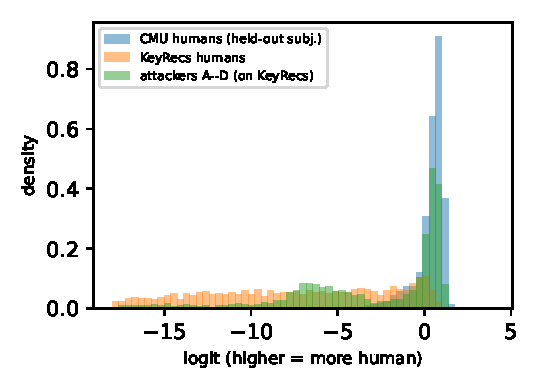
\includegraphics[width=0.9\columnwidth]{../paper_assets/figures/transfer_scores.pdf}
\caption{Typing logits under the CMU-trained model (seed 0). KeyRecs humans fall in the bot range. Their larger dispersion and different per-key means are the likely cause; this was not isolated (Section~\ref{sec:disc}).}
\label{fig:transfer}
\end{figure}
The in-domain controls pass (0.775 for CMU held-out subjects, 0.807 for KeyRecs held-out subjects). Under CMU statistics, the target-humans' DD and flight z-scores have standard deviation 1.7--1.8 (CMU: 1.0). Removing flight features does not fix the result, and per-dataset normalization raises CMU$\to$KeyRecs only to 0.289. For KeyRecs$\to$CMU, per-dataset normalization raises AUC from 0.456 to 0.642. We interpret the below-chance direction as a documented distribution shift, not a sign error or pipeline bug, and we do not claim cross-population transfer.

\subsection{On-device cost (this CPU only)}
\begin{table}[t]
\caption{On-device cost on this CPU (onnxruntime, 1 thread, single session, N=1000). Not a mobile measurement.}
\label{tab:ondevice}
\centering
\small
\begin{tabular}{lccccc}
\toprule
Format & size (KB) & median (ms) & p95 (ms) & $\Delta$AUC vs fp32 & decision agreement \\
\midrule
fp32 ONNX & 267.6 & 0.283 & 0.497 & -- & -- \\
int8 dynamic & 236.7 & 0.302 & 0.672 & +0.0009 & 0.9966 \\
\bottomrule
\end{tabular}
\end{table}

Export to ONNX Runtime and inference on this CPU (one thread, single session, 1000 timed runs) gives median 0.28 ms (fp32, 268 KB) and median 0.30 ms (int8, 237 KB). int8 changes AUC by $+0.0009$ and agrees with fp32 on the decisions reported in Table~\ref{tab:ondevice}; on this CPU it is not faster. These are not mobile or browser measurements.

% ---------------------------------------------------------------------
\section{Discussion and Limitations}
\label{sec:disc}
\textbf{Synthetic positives.} Every ``automated'' session is synthetic. Results quantify performance against the modeled generators, not against real-world fraud.

\textbf{Assumed OTP model.} No public data constrain the OTP-latency densities. Mobile OTP autofill can make very short latencies normal for legitimate users, so the assumed human density may be wrong on such devices; the sensitivity analysis bounds, but does not remove, this risk.

\textbf{Dataset composition.} Per-signal samples come from different populations and are paired synthetically, so inter-signal dependence within an individual is not modeled.

\textbf{Motion domain mismatch.} The motion signal is pocket-worn sit and standing data from MotionSense (24 subjects). It is not hand-held typing motion, and its 50~Hz rate is taken from documentation. Motion results therefore say nothing about how a phone held in the hand behaves during entry. A small number of subjects also means that the motion test fold contains few distinct people, and motion windows are reused across sessions.

\textbf{Epoch cap and convergence.} Training is capped at 24 epochs. The cap binds unevenly across variants (the no-adversarial variant reaches it most often), so part of the difference between adversarial and non-adversarial variants may reflect under-training rather than the adversarial term.

\textbf{Adversarial weight sensitivity.} With the adversarial weight at 1.0 (the same as the BCE term), early stopping selected the first epoch in pilot runs at every perturbation radius we tried. The reported model uses 0.2, a choice made after these pilots, so the adversarial-training results depend on it.

\textbf{Post-hoc exploratory typing variant.} Motivated by the typing-only-bot diagnosis, we trained after the main results an exploratory variant in which six per-session summary statistics of the typing inputs (means and SDs of the hold, DD and flight channels) are concatenated to the typing encoder's final state. This is a post-hoc exploratory variant, not the main model, with seed 0 and five folds, and it was not tuned on test metrics. Its typing-only AUC is \TsFamA{} for family A (main model \OrigFamA{}) and \TsFamB{} for family B (main model \OrigFamB{}), with no gain for the replay and learned families (\TsFamC{} and \TsFamD{}). Its pooled AUC with the OTP term is \TsPooled{}, against \OrigPooledAucP{} for the main model and \GbtPooledAucP{} for GBDT; the intervals overlap. Its ECE is \TsEce{} (main model \OrigPooledEce{}; GBDT \GbtPooledEce{}). A without-OTP version was not trained. Because the variant was chosen after inspecting test-set diagnostics, its gains are optimistic, and they are single-seed.

\textbf{Simple baselines are strong here.} On these synthetic sessions a gradient-boosted tree on hand-crafted features has higher pooled AUC than the no-adversarial neural variant; the paper reports this rather than tuning the neural model against it. Population-level one-class detectors score the naive family as more human than humans: naive bots sit near the centre of the population marginals, so these detectors flag marginal outliers, not interval regularity. We did not reverse their score direction after seeing this.

\textbf{Cross-dataset transfer failed.} A typing-only detector trained on CMU ranks KeyRecs humans as more bot-like than the attackers (AUC 0.25--0.29 across three settings). The reverse direction is at chance without per-dataset normalization (0.44--0.46) and above chance with it (0.64). Both results are single-seed. We do not claim cross-population transfer.

\textbf{Exchangeability.} Conformal guarantees assume exchangeable calibration and test data; adaptive adversaries break this, and coverage on attacked data is measured, not guaranteed.

\textbf{Scope of the task.} The system discriminates human from automated sessions. It does not verify identity, does not detect human fraudsters, and does not detect SIM swap. The SIM-age prefix heuristic is excluded because it cannot be validated without operator ground truth and is confounded by number portability and number recycling.

\textbf{Client integrity.} A score computed entirely in the browser can be forged by a client-controlling adversary. Deployment requires server-side verification or platform attestation, and ``on-device'' processing alone should not be read as a regulatory-compliance argument; we make no legal claim here.

\textbf{Incomplete runs and reduced scope.} Several items were reduced for compute reasons, and the reported numbers reflect this. (i) The 24-epoch training cap was reached by 47\% of no-adversarial runs and 20--27\% of full and no-prior runs. Only the seven capped no-adversarial runs were rerun at 48 epochs, where AUC changed by $+0.004$; the capped full and no-prior runs were not rerun. (ii) The no-OTP habitID-Net result is one seed (five folds); the no-OTP baselines have more seeds where applicable. (iii) Cross-dataset transfer results are single-seed. (iv) The lambda-sweep setting $\lambda_{\text{prior}}=10$ has four folds; its fifth fold was cut before it started. (v) Leave-one-family-out results for habitID-Net are single-seed and have no confidence intervals. (vi) Latency was measured on one CPU thread on the development machine only; no mobile or browser measurement was made. (vii) The bibliography and the related-work claims were not re-verified against their sources. (viii) The paper has not been compiled with a TeX toolchain in this study.

\textbf{Fairness.} We do not measure performance across demographic groups, input methods, or assisted-entry scenarios (e.g., an agent typing for a customer), which may produce atypical timing.

% ---------------------------------------------------------------------
\section{Ethics}
All human data are from public datasets used under their licenses. No personal identifiers are collected; any demonstration of the validity gate uses synthetic numbers. Attacker data are generated synthetically. No human-subject data collection was performed for this study.

% ---------------------------------------------------------------------
\section{Conclusion and Future Work}
We built a prior-regularized, temperature-scaled, conformally thresholded fusion model trained against learned bot generators, and evaluated it with leave-one-family-out, reporting the worst held-out family. The main empirical finding is negative for the neural model: a boosted-tree baseline has higher pooled AUC and lower calibration error, with and without the OTP term. The fused model's higher number is confined to the held-out-family worst case, measured on one seed without confidence intervals. Future work includes validation on real fraud labels through an industry partner, a server-verified architecture with attestation, native-app deployment, and fairness evaluation across devices and populations.

% ---------------------------------------------------------------------
\section*{Acknowledgment}
\TBD{course, instructor, compute resources}

% ---------------------------------------------------------------------
\appendix
\section{Digraph audit}
\label{app:audit}
\begin{table}[t]
\caption{Audit: digraph convention check (Appendix~A of the paper, from the Phase 0 audit).}
\label{tab:audit}
\centering
\small
\begin{tabular}{lccc}
\toprule
Dataset & rows & fraction with standard $\mathrm{UD}=\mathrm{DD}-H(k_1)$ & flight $<0$ (fraction) \\
\midrule
CMU DSL-StrongPasswordData & 20400 & 1.0000 & 0.1084 \\
KeyRecs fixed-text & 19772 & 0.0000 (standard; stored = 0) & 0.0947 (DD$-$H(k1)) \\
KeyRecs free-text & 562372 & 1.0000 & 0.1741 \\
\bottomrule
\end{tabular}
\end{table}


% ---------------------------------------------------------------------
% References: verify every entry (authors, year, venue, pages) before submission.
\begin{thebibliography}{99}

\bibitem{monrose2000}
F.~Monrose and A.~D. Rubin, ``Keystroke dynamics as a biometric for authentication,'' \emph{Future Generation Computer Systems}, vol.~16, no.~4, pp.~351--359, 2000.

\bibitem{killourhy2009}
K.~S. Killourhy and R.~A. Maxion, ``Comparing anomaly-detection algorithms for keystroke dynamics,'' in \emph{Proc. IEEE/IFIP Int. Conf. Dependable Systems and Networks (DSN)}, 2009, pp.~125--134.

\bibitem{dhakal2018}
V.~Dhakal, A.~M. Feit, P.~O. Kristensson, and A.~Oulasvirta, ``Observations on typing from 136 million keystrokes,'' in \emph{Proc. ACM CHI}, 2018.

\bibitem{palin2019}
K.~Palin, A.~M. Feit, S.~Kim, P.~O. Kristensson, and A.~Oulasvirta, ``How do people type on mobile devices? Observations from a study with 37,000 volunteers,'' in \emph{Proc. ACM MobileHCI}, 2019.

\bibitem{acien2022typenet}
A.~Acien, J.~V. Monaco, A.~Morales, R.~Vera-Rodriguez, and J.~Fierrez, ``TypeNet: Deep learning keystroke biometrics,'' \emph{IEEE Trans. Biometrics, Behavior, and Identity Science}, 2022.

\bibitem{acien2021becaptcha}
A.~Acien, A.~Morales, J.~Fierrez, and R.~Vera-Rodriguez, ``BeCAPTCHA: Behavioral bot detection using touchscreen and mobile sensors benchmarked on HuMIdb,'' \emph{Engineering Applications of Artificial Intelligence}, 2021.

\bibitem{frank2013}
M.~Frank, R.~Biedert, E.~Ma, I.~Martinovic, and D.~Song, ``Touchalytics: On the applicability of touchscreen input as a behavioral biometric for continuous authentication,'' \emph{IEEE Trans. Information Forensics and Security}, vol.~8, no.~1, pp.~136--148, 2013.

\bibitem{tey2013}
C.~M. Tey, P.~Gupta, and D.~Gao, ``I can be you: Questioning the use of keystroke dynamics as biometrics,'' in \emph{Proc. NDSS}, 2013.

\bibitem{serwadda2013}
A.~Serwadda and V.~V. Phoha, ``When kids' toys breach mobile phone security,'' in \emph{Proc. ACM CCS}, 2013.

\bibitem{stefan2012}
D.~Stefan, X.~Shu, and D.~Yao, ``Robustness of keystroke-dynamics based biometrics against synthetic forgeries,'' \emph{Computers \& Security}, vol.~31, no.~1, pp.~109--121, 2012.

\bibitem{guo2017}
C.~Guo, G.~Pleiss, Y.~Sun, and K.~Q. Weinberger, ``On calibration of modern neural networks,'' in \emph{Proc. ICML}, 2017.

\bibitem{vovk2005}
V.~Vovk, A.~Gammerman, and G.~Shafer, \emph{Algorithmic Learning in a Random World}. New York: Springer, 2005.

\bibitem{angelopoulos2021}
A.~N. Angelopoulos and S.~Bates, ``A gentle introduction to conformal prediction and distribution-free uncertainty quantification,'' arXiv:2107.07511, 2021.

\bibitem{madry2018}
A.~Madry, A.~Makelov, L.~Schmidt, D.~Tsipras, and A.~Vladu, ``Towards deep learning models resistant to adversarial attacks,'' in \emph{Proc. ICLR}, 2018.

\bibitem{goodfellow2014}
I.~Goodfellow \emph{et al.}, ``Generative adversarial nets,'' in \emph{Proc. NeurIPS}, 2014.

\bibitem{dias2023keyrecs}
T.~Dias, J.~Vitorino, E.~Maia, O.~Sousa, and I.~Pra\c{c}a, ``KeyRecs: A keystroke dynamics and typing pattern recognition dataset,'' \emph{Data in Brief}, vol.~50, p.~109509, 2023.

\bibitem{malekzadeh2019}
M.~Malekzadeh, R.~Clegg, A.~Cavallaro, and H.~Haddadi, ``Mobile sensor data anonymization,'' in \emph{Proc. IoTDI}, 2019. (MotionSense dataset.)

\bibitem{verhoeff1969}
J.~Verhoeff, \emph{Error Detecting Decimal Codes}, Mathematical Centre Tract 29. Amsterdam: Mathematisch Centrum, 1969.

\end{thebibliography}

\end{document}